\chapter{Verifica e validazione}
\label{cap:verifica-validazione}

\intro{In questo capitolo, vengono descritte le scelte riguardanti i test effettuati per verificare e validare il sistema sviluppato. Si inizia con una panoramica delle scelte generali, seguita da una descrizione dei test di unità e dei test specifici per \gls{llm}.}


\section{Scelte riguardanti i test}

Per garantire la qualità del sistema sviluppato, è stato deciso di seguire la pratica dell'ingegneria del software di effettuare test in parallelo allo sviluppo. Questo approccio consente di identificare e correggere i bug in modo tempestivo, migliorando la stabilità e l'affidabilità del sistema.

Tuttavia, essendo il sistema molto semplice, in particolare considerato l'approccio procedurale con la conseguente assenza di classi, si è deciso di non implementare l'intera suite di test automatizzati prevista dalla teoria (test di unità, test di integrazione, test di sistema, test di accettazione). Invece, si è optato per un approccio più snello, concentrandosi sui test di unità.

Tuttavia, considerando l'importanza della qualità delle risposte del modello \gls{llm} utilizzato, il fallimento del quale comporterebbe il fallimento totale del sistema, sono stati implementati test specifici per verificare il corretto funzionamento del modello stesso. Questi test, a differenza dei test di unità, non utilizzano un mock per il modello \gls{llm}, ma bensì si basano sul modello reale utilizzato in produzione.

Inoltre, durante lo sviluppo delle interfacce frontend, nonostante non fosse richiesto, si è comunque deciso di implementare dei test per verificare il corretto funzionamento dei componenti, essendo una buona pratica dello sviluppo software in generale.


\section{Test di unità}

I test di unità sono stati implementati per verificare il corretto funzionamento delle singole funzioni e moduli del sistema. Per ogni file di codice sorgente, è stato scritto un corrispettivo file di test, emulando la stessa struttura di cartelle. Questi test sono stati scritti utilizzando i seguenti framework:
\begin{itemize}
    \item \textbf{pytest}: framework di testing per Python che offre una sintassi semplice e intuitiva. Permette di scrivere test con asserzioni standard di Python e fornisce funzionalità avanzate come fixture, parametrizzazione dei test e un sistema di plugin estensibile;
    \item \textbf{unittest}: modulo standard di Python per il testing unitario, basato sul framework xUnit. Utilizza una struttura orientata agli oggetti dove i test sono definiti come metodi di classi che ereditano da \texttt{unittest.TestCase}.
\end{itemize}

È stato poi scelto, per ciascuna function, di scrivere un file \texttt{pytest.ini} per configurare il framework \texttt{pytest} per calcolare la copertura del codice ad ogni esecuzione dei test. Questo file contiene le impostazioni per il calcolo della copertura del codice, specificando le directory e i file da includere o escludere dal report di copertura. È stata decisa, di comune accordo con il tutor, una copertura minima del 90\% per ogni file di codice sorgente, in modo da garantire un buon livello di test e ridurre il rischio di bug non rilevati.

Alla fine, è stata ottenuta una copertura del codice del 100\% per tutti i file di codice sorgente di entrambe le functions, il che significa che ogni riga di codice è stata eseguita almeno una volta durante i test. Questo è un risultato molto positivo, poiché indica che tutte le funzionalità implementate sono state testate e verificate.
Questo risultato è stato riportato tramite badge nel \texttt{README.md} del repository, come visibile nella figura \ref{fig:coverage-badges}, in modo da fornire una visione chiara della qualità del codice e della copertura dei test.

\begin{figure}
    \centering
    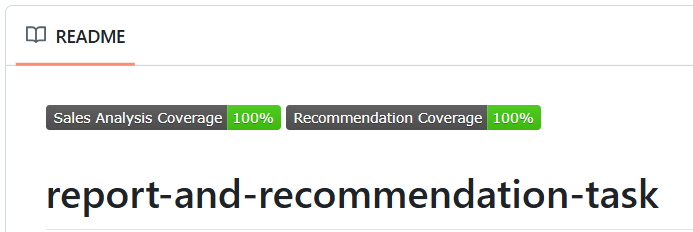
\includegraphics[width=0.8\textwidth]{Badges di coverage delle functions.png}
    \caption{Badge di copertura del codice per le functions}
    \label{fig:coverage-badges}
\end{figure}


\section{Test dell’LLM}

Per garantire la qualità delle risposte fornite dal modello \gls{llm} utilizzato, sono stati implementati test specifici per verificare il corretto funzionamento del modello stesso. Questi test sono stati scritti utilizzando il framework \texttt{pytest} e si basano sul modello reale utilizzato in produzione, senza l'utilizzo di mock.

Inoltre, siccome l'\gls{llm} è un servizio a pagamento, per evitare di spendere denaro ad ogni esecuzione dell'intera suite di test, è stato deciso di marcare appositamente questi test con il decoratore \texttt{pytest.mark.llm}, e, soprattutto, è stato configurato \texttt{pytest} per escludere tale decoratore dall'esecuzione principale prevista dal comando \texttt{pytest}.
In questo modo, è possibile eseguire solo i test relativi al modello \gls{llm} quando necessario, utilizzando il comando \texttt{pytest -m llm}, ed è possibile eseguire i test rimanenti con il normale comando \texttt{pytest} senza dover pagare alcunchè.

L'\gls{llm} viene chiamato due volte nel sistema: una volta per riconoscere le colonne dentro il file CSV e una volta per generare un resoconto delle statistiche e dei grafici del report delle vendite. Per ciascuna di queste chiamate, sono stati implementati test specifici con vari differenti input per verificare che il modello risponda correttamente e che le risposte siano coerenti con le aspettative.


\section{Test del frontend}

Durante lo sviluppo delle interfacce frontend, sono stati implementati test per verificare il corretto funzionamento dei componenti. 

Come framework di test, sono state valutate le seguenti possibilità:
\begin{itemize}
    \item \textbf{Jest}: un framework di test JavaScript sviluppato da Facebook, ampiamente utilizzato per testare applicazioni React. Offre funzionalità come snapshot testing, mocking e copertura del codice;
    \item \textbf{Vitest}: un framework di test moderno e veloce per JavaScript e TypeScript, progettato per essere compatibile con Jest. Supporta il testing di componenti React e offre funzionalità simili a Jest.
\end{itemize}

Siccome le applicazioni React sviluppate si basano su Vite, un moderno strumento di build per applicazioni web, si è deciso di utilizzare Vitest come framework di test. Vitest è progettato per essere veloce e leggero, sfruttando le stesse tecnologie di Vite, e offre una sintassi simile a Jest, rendendo facile la scrittura e l'esecuzione dei test.

Per entrambi i progetti frontend, è stato deciso di non fissare a priori una copertura minima del codice, ma di puntare bensì a testare le funzionalità principali e i casi d'uso più rilevanti. Questo approccio consente di mantenere un buon livello di test senza appesantire lo sviluppo con requisiti di copertura troppo rigidi.
Nel caso del frontend di analisi delle vendite, è stato comunque ottenuto un buon livello di copertura del codice, con una copertura pari al 62\%. Per il frontend di raccomandazione invece, a causa di un diverso approccio nell'uso dei mock che non ha previsto l'usufrutto del codice dei tipi di dato \texttt{Shadcn/ui} (i quali sono considerati tra le righe di codice da coprire pur essendo stati generati automaticamente), la coverage è stata ottenuta pari al solo 34\%. Tuttavia, anche in questo caso, i componenti principali e le funzionalità più rilevanti sono stati testati, garantendo un buon livello di affidabilità.
